
\chapter{Aprendizaje Automático}
\label{chap:Aprendizaje-Automatico}

\section{Introducción}
En el contexto de aprendizaje automático, los patrones deben ser descubiertos a partir de una serie de muestras que son denominadas instancias. El conjunto de entrada se denomina conjunto de entrenamiento. En nuestro caso específico, cada instancia es un vector de características extraída de señales en una determinada ventana de tiempo. Las muestras en el conjunto de entrenamiento pueden o no ser etiquetadas, es decir, tener asociada a una clase conocida (por ejemplo, caminar, correr, etc.). En algunos casos, tener datos etiquetados no es factible, ya que puede requerir un experto para examinar manualmente los ejemplos y asignar una etiqueta en base a su experiencia.

El proceso de aprendizaje es generalmente tedioso, caro y consume mucho tiempo en muchas aplicaciones de minería de datos. Existen dos enfoques de aprendizaje, es decir, aprendizaje supervisado y no supervisado, que se ocupan de datos etiquetados y no etiquetados, respectivamente. Puesto que un sistema de reconocimiento de la actividad humana debe devolver un resultado como caminar, sentarse, correr, etc., la mayoría de los sistemas de \abbr{HAR} utilizan algoritmos de aprendizaje supervisados. De hecho, podría ser muy difícil de discriminar actividades en un contexto completamente sin supervisión. Algunos otros sistemas funcionan de una manera semisupervisada en donde parte de los datos están sin etiqueta.

Muchos autores definen aprendizaje automático de distintas maneras, aunque \cite{Murphy:2012:MLP:2380985} lo define de manera muy clara:

\vspace{5mm}

\begin{definition}[Aprendizaje Automático (\emph{Machine Learning}, \abbr{ML})] 
    \label{def3:ml}Definimos el aprendizaje automático como un conjunto de métodos que pueden detectar automáticamente patrones en los datos y luego utilizar estos patrones descubiertos para predecir los datos futuros o para realizar otros tipos de toma de decisiones bajo incertidumbre.
\end{definition}

\section{Aprendizaje Supervisado}

\label{sec3:aprendizaje}De manera a establecer un marco teórico para los algoritmos de aprendizaje automático supervisados \cite{Rajaraman2011} se incluye la siguiente definición formal.

\begin{definition}[Clasificador (\emph{Machine Learning}, \abbr{ML})]\label{def3:clasificacion}Un algoritmo \abbr{ML} recibe un conjunto entrenamiento que se compone de varios pares $(\boldsymbol{x},y)$ conocidos como instancias de entrenamiento, donde
\begin{itemize}
\item $\boldsymbol{x}$ es un \emph{vector} de valores, llamado vector característico, e
\item $\boldsymbol{y}$ es la \emph{etiqueta}, el valor de clasificación para $\boldsymbol{x}$.
\end{itemize}
El objetivo del proceso \abbr{ML} es encontrar una función $y=f(\boldsymbol{x})$ cuya predicción de $\boldsymbol{y}$ asociada a valores desconocidos de $\boldsymbol{x}$ sea la mejor. El valor de $\boldsymbol{y}$ corresponde a valores arbitrarios pero es común encontrase con los siguientes casos:
\begin{enumerate}
\item $\boldsymbol{y}$ es un número del conjunto de los reales. Este caso corresponde a un problema de regresión.
\item $\boldsymbol{y}$ es un valor booleano verdadero-falso, también representado como $+1$ y $-1$. Este caso corresponde a una clasificación binaria. 
\item $\boldsymbol{y}$ es miembro de un conjunto finito discreto donde cada valor representa una clase particular. El problema es llamado de clasificación de múltiples clases.
\end{enumerate}
\end{definition}

El aprendizaje supervisado, comúnmente conocido como clasificación de múltiples clases discretas, ha sido un campo muy productivo que da lugar a un gran número de algoritmos. En la \tabref{tab3:clasificadores} se resumen los clasificadores más importantes en el estudio de \abbr{HAR}s según su tipo.
\begin{table}[!htbp]
\begin{centering}
\begin{tabular}{|l|l|}
\hline 
		Tipo 						& Clasificador							\\
\hline 
\hline 
		Arboles de Decisión 		& C4.5, ID3								\\
\hline 
		Clasificadores de Bayes 	& Redes de Bayes, \emph{Naïve} Bayes	\\
\hline 
		Basados en Instancia 		& k-vecinos proximos					\\
\hline 
		Transformación de dominio 	& Máquinas de soporte-vector			\\
\hline 
		Redes neuronales 			& Perceptron de múltiples capas			\\
\hline 
		Modelos de Markov 			& Modelos ocultos de Markov				\\
\hline
\end{tabular}
\par\end{centering}
\caption[Algoritmos de ML]{\label{tab3:clasificadores} Algoritmos de aprendizaje automático}
\end{table}

En las siguientes secciones nos concentraremos en un enfoque basado en arboles de decisión (\emph{Decision Tree}, \abbr{DT}) para construir la función $f$. La función $f$, que corresponde a un árbol de múltiples niveles donde cada nodo aplica una función a $\boldsymbol{x}$ y determina sobre qué nodo hijo procede la búsqueda. Cada nodo posee un número arbitrario de nodos hijos. Los árboles de decisión son preferibles para las clasificación binaria o de múltiples clases, especialmente cuando la dimensión del vector característicos no es muy grande \cite{Rajaraman2011}.

\section{Arboles de Decisión}
El árbol de decisión es un método de aprendizaje predictivo sobre un conjunto de tuplas o instancias etiquetadas. Un árbol de decisión es una estructura de árbol similar a un diagrama de flujo, donde cada nodo interno (nodo no hoja) denota una prueba de un atributo, y cada rama representa el camino de a seguir luego de la evaluación, y cada nodo hoja es una etiqueta o clase.

\begin{figure}[!htbp]
	\centering
	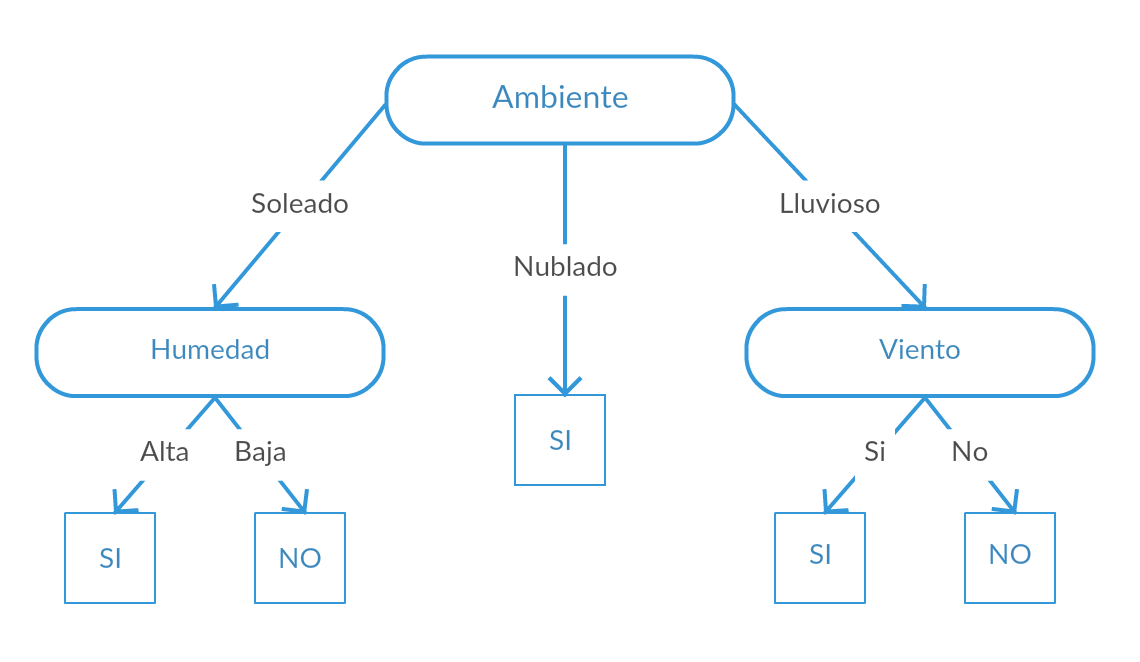
\includegraphics[width=0.7\linewidth]{capitulo-3/graphics/ad_2}
	\caption[Ejemplo de árbol de decisión]{\label{fig:arbolEjemplo}Árbol de decisión}
\end{figure}

En la \figref{fig:arbolEjemplo} se muestra un típico ejemplo de árbol de decisión que representa el concepto de jugar o no Golf, teniendo en cuenta variables climática representadas en los nodos internos, y los nodos hojas denotan las decisiones de jugar o no al Golf. 

\section{Algoritmo C4.5}
El trabajo de J.R. Quinlan \cite{Quinlan:1993:CPM:152181} propone un algoritmo de construcción de arboles de decisión denominado C4.5, el cual a su vez es una mejora o extensión al algoritmo ID3 \cite{Quinlan:1986:IDT:637962.637969}. Este algoritmo genera un árbol de decisión a partir del paticionamiento recursivo de los datos de entrada. El árbol se construye mediante la estrategia \emph{profundidad-primero (depth-first)}.

Además, el algoritmo C4.5 utiliza una técnica heurística conocida como \emph{proporción de ganancia (gain-ratio)}. Que es una medida basada en información que considera diferentes números y probabilidades de los resultados de las pruebas. El algoritmo así, considera todas las pruebas posibles que puede dividir el conjunto de datos para seleccionar la prueba que le haya generado mayor ganancia de información. Para cada atributo discreto, se considera una prueba con $N$ resultados, siendo $N$ el numero de valores posibles que puede tomar el atributo. Para cada atributo continuo, se realiza la prueba binaria (1, 0) sobre cada uno de los valores que puede tomar el atributo de los datos. 

El algoritmo C4.5, ilustrado en el Algoritmo \ref{algoC45}, presenta las siguientes características:

\begin{itemize}
	\item Permite trabajar con valores continuos para los atributos, en dos ramas según se cumpla una de las siguientes condiciones  $ A_{i} <= N $ o $ A_{i} > N $ . 
	\item Por lo general los arboles generados por el mismo se caracterizan por ser menos frondosos, ya que cada hoja cubre una distribución de clases y no una clase en particular.
	\item Utiliza el método \emph{divide y vencerás} para generar el árbol de decisión inicial a partir de un conjunto de datos de entrenamiento.
	\item Se basan en la utilización del criterio de proporción de ganancia, definido como $ I(X_{i},C) / I(X_{i})  $. De esta manera consigue evitar que variables con mayor numero de categorías salgan beneficiadas en la selección. 
	\item Su implementación típica es recursiva.
\end{itemize}

\begin{algorithm}
	\begin{algorithmic}[1]
		\Require Conjunto de datos etiquetados $D$
		\Procedure{C4.5}{$ D $}
			\If {$D > \textit{es puro o cumple el criterio de parada} $} 
				\State\textit{Termina}
			\EndIf
			\ForAll{$a \in D $}
				\State $\textit{Computar información de division en a }$
			\EndFor
			\State $ a_{best} =$ Mejor atributo de división respecto al criterio 
			\State $ Arbol =$ Crear un nodo de decisión con $ a_{best} $ en la raíz 
			\State $ D_{v} =$ Introducir sub-conjunto de $D$ basado en división $ a_{best} $
			\ForAll{$ D_{v} $}
				\State $ Arbol_{v} = C4.5(D_{v}) $
				\State Unir $ Arbol_{v} $ al correspondiente arco del Árbol
			\EndFor
			\State 
			\Return $ Arbol $
		\EndProcedure
	\end{algorithmic}
	\caption{\label{algoC45}Algoritmo C4.5}
\end{algorithm}


\section{Selección de Atributo de División}
Las medidas de selección de atributos de división se utilizan heurística para seleccionar el criterio de división que mejor separa una partición de datos dada $D$ de tuplas de entrenamiento etiquetadas en clases individuales. Si dividimos $D$ en particiones más pequeñas de acuerdo a un criterio de división dado, idealmente tendríamos cada partición pura, es decir todas la tuplas deben permaneces a la misma clase. Por lo tanto, el mejor medida de selección de atributo es el que se acerque más al escenario mencionado.

La medida de selección de atributo también se conocen como reglas de división porque determinan como se dividen las tuplas en un nodo determinado. Esta proporciona un rating para cada atributo de la tupla de entrenamiento. El atributo con mejor valor en esta medida es el elegido como atributo de división. Si el atributo de división es de valor continuo, el árbol sera binario, también debe determinarse el punto de división o un subconjunto de división como parte del criterio de división.

El nodo raíz es creado para la partición $D$ etiquetado con el criterio de división, se crean ramas para cada resultado del criterio de división, y las tuplas se dividen en consecuencia. 

De aquí en adelante, utilizaremos la siguiente nomenclatura. Sea $D$ una partición de datos, un conjunto de tuplas de entrenamiento etiquetadas. Supongamos que la clase tiene $m$ valores distintos, que definen $m$ clases distintas $C_i$ (Siendo $i=1,..,m$). De modo que $C_{i,D}$ es el conjunto de tuplas de la clase $C_{i}$ en $D$. Por lo tanto $\lvert D \rvert$ y $\lvert C_{i,D} \rvert$ denotan la cantidad de tuplas en $D$ y $C_{i,D}$ respectivamente. 

\subsection{Información de ganancia / entropía}
El algoritmo ID3 utilizan la entropía como medida de selección para cada atributo.
En donde, dado un nodo $N$ que representa las tuplas de la partición $D$, el atributo con mayor valor de ganancia es elegido para la división de $N$. Con este enfoque, el atributo reduce al mínimo la información necesaria para clasificar las tuplas de las particiones resultantes y refleja la menor aleatoriedad o impureza de la partición. Este enfoque minimiza el número esperado de ensayos necesarios para clasificar una tupla dada y garantiza un que se encuentre un árbol simple, pero no necesariamente el arbol más simple.

La información de ganancia necesaria para clasificar una tupla en $D$ está dada por:

\begin{equation}
Info(D) = - \displaystyle\sum_{i=1}^{m} p_{i}\log_2(p_{i})\label{eq3:info}
\end{equation}

donde $p_{i}$ es la probabilidad de una tupla arbitraria en $D$ pertenezca a la clase $C_{i}$ y que se estima que es igual a $ \lvert C_{i,D}} \rvert / \lvert D \rvert $. $Info(D)$ es la cantidad media de información necesaria para identificar la etiqueta de una tupla dada en $D$. Nótese, que la información que tenemos se basa solamente en las proporciones de las tuplas de cada clase. $Info(D)$ también se conoce entonces como entropía de $D$.

Ahora, supongamos que se requiera particionar las tuplas en $D$ conforme a los atributos $A$ conformados por $v$ valores distintos $ \{ a_{1},a_{2},...,a_{v} \}$. Si $A$ tiene valores discretos, estos valores se corresponderán directamente con los resultados de una prueba de $v$ sobre $A$. El atributo $A$ se puede utilizar para dividir $D$ en $v$ particiones o subconjuntos, $ \{ D_{1},D_{2},...,D_{v} \}$, donde $D_j$ contiene aquellas tuplas en $D$ que se corresponden con $a_j$ resultados de $A$. Estas particiones se corresponderían con las ramas que crecen a partir del nodo $N$. Idealmente, nos gustaría que esta división pueda producir una clasificación exacta de las tuplas. Es decir, nos gustaría que cada partición sea pura. Sin embargo, es bastante probable que el particionamiento sea impuro (por ejemplo, cuando una partición puede contener una colección de tuplas de diferentes clases en lugar de una sola clase). ¿Cuánto más información sería todavía necesaria (luego de la partición) con el fin de llegar a una clasificación exacta? Esta cantidad se mide por:

\begin{equation}
Info_{A}(D) = \displaystyle\sum_{j=1}^{v} \displaystyle\frac{\lvert D_{j} \rvert}{\lvert D \rvert} \times Info(D_{j})\label{eq3:infoA}
\end{equation}

El termino $\displaystyle\frac{\lvert D_{j} \rvert}{\lvert D \rvert}$ actúa como el peso de la j-esima partición. $Info_{A}(D)$ es la información esperada requerida para clasificar la tupla de $D$ basada en la partición de $A$. Cuando menor sea la información esperada, mayor es la pureza de las particiones.

La información de ganancia se define como la diferencia entre lo requerido de información original (basado en la proporción de clases) y el nuevo requerimiento, obtenido luego de realizar la partición en $A$. Es decir,

\begin{equation}
Gain(A) = Info(D) - Info_{A}(D)\label{eq3:ganancia}
\end{equation}

En otras palabras, $Gain(A)$ nos dice cuanto se ganaría por la ramificación en $A$. Es la reducción esperada en el requisito de información causado por conocer el valor de $A$. El atributo A con ganancia mas alta, $Gain(A)$, se selecciona como atributo de división en el nodo $N$. Esto equivale a decir que queremos particionar en el atributo A que haría la mejor clasificación, por lo que la cantidad de información aun necesaria para clasificar las tuplas sea mínima, $InfoA(D)$.

\subsection{Ejemplo de deducción de un nodo - ID3}

En la siguiente \tabref{tabla:sencilla2} se presenta un conjunto de entrenamiento $D$, con la clase etiquetada, de una base de datos de compra de productos electrónicos. Para este ejemplo, cada atributo tiene un valor discreto, y los atributos de valores continuos fueron generalizados. La clase \textit{Compra Computador} tiene dos valores posibles: $SI$ y $NO$, y por lo tanto existen dos clases distintas (es decir, $m=2$). Por lo tanto, tenemos la clase $C_1$ que corresponde a $SI$ y la clase $C_2$ corresponde a $NO$.

Existen nueve tuplas de la clase $SI$, y cinco de la clase $NO$. Para encontrar el criterio de división para las tuplas debemos calcular la ganancia de información de cada atributo. Primero usamos la ecuación \ref{eq3:info} para calcular la información esperada necesaria para clasificar una tupla en $D$:

\begin{equation*}
Info(D) = - \frac{9}{14}\log_2(\frac{9}{14}) - \frac{5}{14}\log_2(\frac{5}{14})	= 0.940 bits
\end{equation*}

\begin{table}[!htbp]
	\begin{tabular}{|c|l|l|l|l|c|}
		\hline 
		\textbf{Rid} & \textbf{Edad}    & \textbf{Ingreso} & \textbf{Estudiante} & \textbf{Rating Crediticio} & \textbf{Compra Computador?} \\
		\hline 
		\hline
		1   & Joven   & Alto    & No         & Justa             & NO                 \\ 
		2   & Joven   & Alto    & No         & Excelente         & NO                 \\ 
		3   & Mediana & Alto    & No         & Justa             & SI                 \\ 
		4   & Adulto  & Medio   & No         & Justa             & SI                 \\ 
		5   & Adulto  & Bajo    & Si         & Justa             & SI                 \\ 
		6   & Adulto  & Bajo    & Si         & Excelente         & NO                 \\ 
		7   & Mediana & Bajo    & Si         & Excelente         & SI                 \\ 
		8   & Joven   & Medio   & No         & Justa             & NO                 \\ 
		9   & Joven   & Bajo    & Si         & Justa             & SI                 \\ 
		10  & Adulto  & Medio   & Si         & Justa             & SI                 \\
		11  & Joven   & Medio   & Si         & Excelente         & SI                 \\
		12  & Mediana & Medio   & No         & Excelente         & SI                 \\
		13  & Mediana & Alto    & Si         & Justa             & SI                 \\
		14  & Adulto  & Medio   & No         & Excelente         & NO                 \\
		\hline
		\hline
	\end{tabular}
	\caption{\label{tabla:sencilla2}Ejemplo de conjunto de entrenamiento considerado}
\end{table}

Luego, necesitamos calcular la información requerida por cada atributo. Comenzamos con el atributo $Edad$, necesitamos observar la distribución de $SO$ y $NO$ por cada categoría o valor de este atributo. Para la categoría $Joven$, hay dos tuplas $SI$ y tres tuplas $NO$. Para la categoría $Mediana$, hay cuatro tuplas $SI$ y cero tuplas $NO$. Para la categoría $Adulto$, hay tres tuplas $SI$ y dos tuplas $NO$. Usando la ecuación \ref{eq3:infoA}, la información esperada necesaria para clasificar una tupla en $D$ si las tuplas son divididas según el atributo $Edad$ corresponde a:

\begin{equation*}
\begin{split}
Info_{Edad}(D) & = \frac{5}{14} \times ( -\frac{2}{5}\log_2(\frac{2}{5})-\frac{3}{5}\log_2(\frac{3}{5})  ) \\
			   & + \frac{4}{14} \times ( -\frac{4}{4}\log_2(\frac{4}{4})-\frac{0}{4}\log_2(\frac{0}{4})  ) \\
			   & + \frac{5}{14} \times ( -\frac{3}{5}\log_2(\frac{3}{5})-\frac{2}{5}\log_2(\frac{2}{5})  ) \\
			   & = 0.694 bits.
\end{split}
\end{equation*}

Por lo tanto, la ganancia esperada de realizar tal partición seria de acuerdo a la ecuación \ref{eq3:ganancia}:

\begin{equation*}
Gain(Edad) = Info(D) - Info_{Edad}(D) = 0.940 - 0.694 = 0.246 bits
\end{equation*}

De la misma manera, se procede a calcular las ganancias para cada atributo:
\begin{itemize}
  \item $Gain(Ingreso)$ = 0.029 bits, 
  \item $Gain(Estudiante)$ = 0.151 bits, y 
  \item $Gain(RatingCrediticio)$ = 0.048 bits. 
\end{itemize}

Dado que el atributo $Edad$ tiene mayor ganancia de información, es seleccionado para realizar la partición. El nodo $N$ es etiquetado con $Edad$, y se crean una rama por cada valor del atributo. Las tuplas se divinen en consecuencia, como se muestra en la \figref{fig:arbolPartEdad}.

\begin{figure}[!tbph]
	\centering
	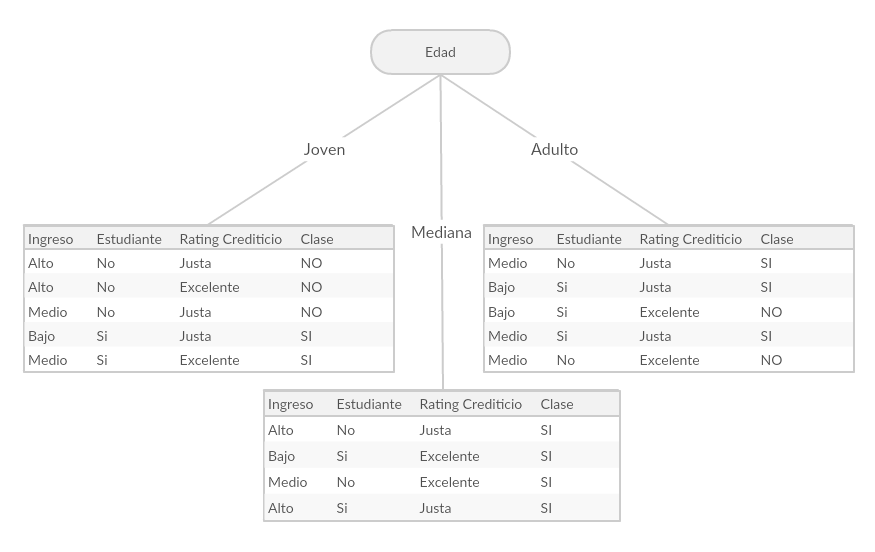
\includegraphics[width=0.7\linewidth]{capitulo-3/graphics/dtree_parti}
	\caption[Árbol de decisión particionado]{\label{fig:arbolPartEdad}Árbol de decisión: Particionado en el atributo 'Edad'}
\end{figure}

Notese que las tuplas en la partición $Edad = Mediana$ pertenecen todas a la clase $SI$, por lo tanto en esta rama se crea una hoja con etiqueta $SI$. Para las particiones $Edad = Joven$ y $Edad = Adulto$, el proceso de deducción se continua hasta que se generen nodos hoja que clasifican las tuplas en una sola clase. El
 árbol de decisión final deducido mediante algoritmo C4.5 se muestra en la \figref{fig:arbolFinal}.
 
\begin{figure}[!tbph]
	\centering
	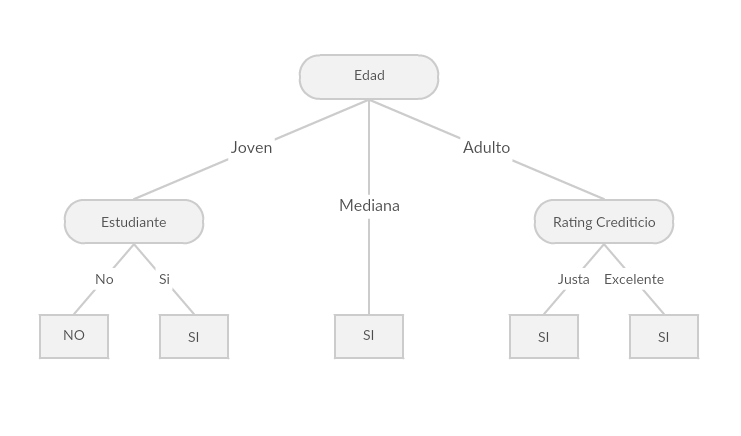
\includegraphics[width=0.7\linewidth]{capitulo-3/graphics/dtree_parti_final}
	\caption[Árbol de decisión final]{\label{fig:arbolFinal}Árbol de decisión final: Luego de finalizar el proceso del C4.5 }
\end{figure}


\subsection{Proporción de ganancia}
La medida de información de ganancia tiene inclinación hacia un particionamiento con muchos resultados, es decir, es propenso a seleccionar atributos que tengan gran numero de valores. Por ejemplo, considerando un atributo que actúa como identificador, como $Rid$; una división en $Rid$ generaría un gran numero de particiones, tantas como valores contenga $Rid$, cada partición con una sola tupla. Debido a que cada partición es pura, la información necesaria para clasificar el conjunto dado $D$ basado en el particionamiento mencionado seria $Info_{Rid}(D)=0$. Por lo tanto, la información de ganancia es la máxima, claramente, tal partición es inútil para la clasificación. 

El algoritmo C4.5, sucesor de ID3, usa una extensión de la información de ganancia conocida como proporción de ganancia, que intenta contrarrestar la inclinación mencionada.	Aplica una normalización a la información de ganancia usando un valor "Informacion de division" definido de manera análoga a $Info(D)$.

\begin{equation}
SplitInfo_{A}(D) = -\displaystyle\sum_{j=1}^{v} \displaystyle\frac{\lvert D_{j} \rvert}{\lvert D \rvert} \times Info(\frac{\lvert D_{j} \rvert}{\lvert D \rvert})\label{eq3:SplitInfo}
\end{equation}

Este valor representa la información potencial generada al dividir el conjunto de datos de entrenamiento $D$ en $v$ particiones, correspondientes a los $v$ de una prueba en el atributo $A$.
Nótese que, para cada resultado, es considerado el numero de tuplas que tienen ese resultado, respecto al numero total de tuplas en $D$. Esto difiere de información de ganancia, que media la información respecto a la clasificación generada basada en la misma partición. La proporción de ganancia se define como:

\begin{equation}
GainRatio(A) = \frac{Gain(D)}{SplitInfo_{A}(D)}\label{eq3:GainRatio}
\end{equation}

El atributo con mayor proporción de ganancia es seleccionado como atributo de división. Tener en cuenta, por otro lado, que a medida que la información de división se acerca a cero, la relación se vuelve inestable. 

\subsection{Ejemplo de deducción de un nodo - C4.5}
De la misma manera que el ejemplo anterior, utilizando la \tabref{tabla:sencilla2}, por ejemplo para el atributo $Ingreso$ una prueba de división divide la tabla en tres particiones, es decir, $alto$, $medio$, $bajo$, las cuales contienen, cuanto, seis, y cuatro tuplas respectivamente. Con estos datos, para calcular la proporción de ganancia del atributo $Ingreso$, debemos calcular primeramente la información de división, utilizando la formula \ref{eq3:SplitInfo}:


\begin{equation*}
SplitInfo_{ingreso}(D) = & - \frac{4}{14} \times \log_2(\frac{4}{14}) \\
						 & - \frac{6}{14} \times \log_2(\frac{6}{14}) \\
						 & - \frac{4}{14} \times \log_2(\frac{4}{14}) \\
						 & = 0.926 bits.
\end{equation*}

Tomando del ejemplo anterior, la información de ganancia $Gain(Ingreso)$ = 0.029 bits, la proporción de ganancia la calcularíamos:

\begin{equation*}
GainRatio(Ingreso) = \frac{0.029}{0.926} = 0.031 bits \\
\end{equation*}



\section{Métricas de Evaluación y Matriz de Confusión}
En general, la selección del algoritmos de clasificación para HAR ha sido apoyada meramente por evidencias empíricas (referencias). La gran mayoría de los estudios utilizan una validación cruzada con pruebas estadísticas para comparar el rendimiento de los clasificadores para un conjunto de datos determinado, como se visualiza en la \figref{fig:evaluacion}.

\begin{figure}[!tbph]
	\centering
	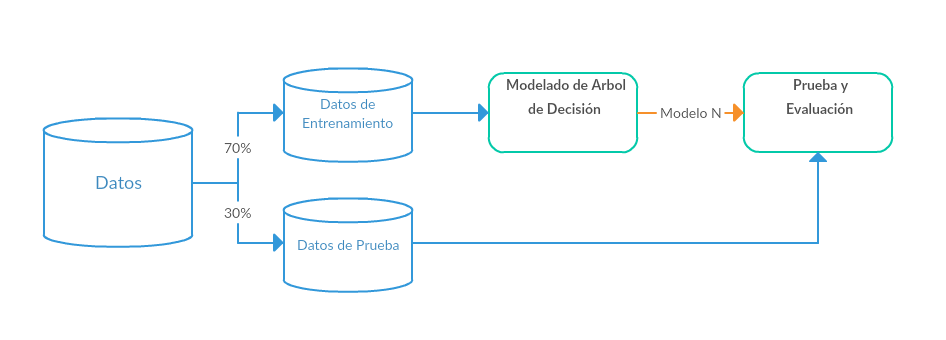
\includegraphics[width=0.7\linewidth]{capitulo-3/graphics/training-test}
	\caption[Diagrama de evaluación de clasificación]{\label{fig:evaluacion}Diagrama de Evaluación de Clasificación}
\end{figure}
	
Los resultados de una clasificación de un método en particular se suelen organizar en una matriz de confusión $M_{n \times n}$ para un problema de clasificación con $N$ clases.
En esta matriz, el elemento $M_{ij}$ es el numero instancias de la clase $i$ que fueron clasificados en la clase $j$.
Los siguientes valores se pueden obtener de la matriz de confusión en un problema de clasificación primaria:

\begin{itemize}
	\item Verdaderos Positivo (\emph{True Positive}, \abbr{TP}): El número de casos positivos que fueron clasificados como positivos.
	\item Verdaderos Negativo (\emph{True Negative}, \abbr{TN}): El número de casos negativos que fueron clasificados como negativos.
	\item Falso Positivo (\emph{False Positive}, \abbr{FP}): El número de casos negativos que fueron clasificados como positivos.
	\item Falso Negativo (\emph{False Negative}, \abbr{FN}): El número de casos positivos que fueron clasificados como negativos.
\end{itemize}

La precisión es la métrica más utilizada para resumir el rendimiento general de la clasificación para todas las clases y se define de la siguiente manera:

\begin{equation}
Exactitud = \frac{TP + TN}{TP + TN + FP + FN}\label{eq3:exactitud}
\end{equation}

La precisión, a menudo denominada valor predictivo positivo, es la proporción de casos positivos clasificados correctamente al número total de casos clasificados como positivos:
\begin{equation}
\mbox{Precisión} = \frac{TP}{TP + FP}\label{eq3:precision}
\end{equation}

La exhaustividad, también llamado tasa positiva verdadera, es la proporción de instancias positivas correctamente clasificadas al número total de instancias positivas:
\begin{equation}
Exhaustividad = \frac{TP}{TP + FN}\label{eq3:exaustividad}
\end{equation}


El Valor-F combina precisión y exhaustividad en un solo valor:
\begin{equation}
Valor-F = 2 \cdot \frac{\mbox{Precisión} \cdot Exhaustividad}{\mbox{Precisión} + Exhaustividad}\label{eq3:valorf}
\end{equation}

Aunque se definen para la clasificación binaria, estas métricas pueden generalizarse para un problema con $N$ clases. En tal caso, una instancia podría ser positiva o negativa según una mejor clase particular, por ejemplo, los positivos podrían ser todas las instancias de ejecución mientras que los negativos serían todas las instancias distintas de la ejecución.

\section{Evaluación de un Modelo}

Utilizando el ejemplo anterior en la \tabref{tabla:sencilla2}, supongamos que se tomo una muestra de 10.000 tuplas obteniendose como resultado la \tabref{tabla:MatrizConfusion}.


\begin{table}[!htbp]
	\begin{tabular}{|l|c|c|c|}
		\hline 
		\textit{Clase} & \textit{Com. Computador = SI}    &\textit{Com. Computador = NO} & \textit{Total}  \\
		\hline 
		\textit{Com. Computador = SI}	& 6.954   	& 46    	& 7.000     \\ 
		\hline 
		\textit{Com. Computador = NO}	& 412		& 2.588		& 3.000    	\\ 
		\hline
		\textit{Total}					& 7.366		& 2.634    	& 10.000	\\ 
		\hline
	\end{tabular}
    \caption{\label{tabla:MatrizConfusion}Matriz de Confusión}
\end{table}


Al evaluar la clase \textit{Compra Computador = SI} tenemos lo siguiente:

\begin{itemize}
	\item Verdaderos Positivo (\abbr{TP}): 6.954
	\item Verdaderos Negativo (\abbr{TN}): 2.588
	\item Falso Positivo (\abbr{FP}): 412
	\item Falso Negativo (\abbr{FN}): 46
\end{itemize}

A partir de estos datos podemos calcular el resto de las métricas:
\begin{equation*}
Exactitud = \frac{TP + TN}{TP + TN + FP + FN} = \frac{6.954 + 2.588}{6.954 + 2.588 + 412 + 46} = \frac{9542}{10000} = 0,9542
\end{equation*}

\begin{equation*}
\mbox{Precisión} = \frac{TP}{TP + FP} = \frac{6.954}{6.954 + 412} = 0,9440
\end{equation*}

\begin{equation*}
Exhaustividad = \frac{TP}{TP + FN} = \frac{6.954}{6.954 + 46} = 0,9934
\end{equation*}

\begin{equation*}
Valor-F = 2 \cdot \frac{\mbox{Precisión} \cdot Exhaustividad}{\mbox{Precisión} + Exhaustividad} 
		= 2 \cdot \frac{\mbox{0,9440} \cdot 0,9934}{\mbox{0,9440} + 0,9934}
		= 0,9680
\end{equation*}

Teniendo en cuenta estas métricas para la muestra de 10.000 tuplas, podemos suponer el que modelo generado de ejemplo tiene unos altos valores de exactitud, precisión, y exhaustividad, lo cual se puede apreciar por la baja tasa de falsos positivos y negativos. Respecto al Valor-F, el tener valores altos de precisión y exhaustividad, da un valor muy alto, ya que el Valor-F es de forma general la media armónica de ambos.

